
%\lipsum[1]

	\begin{figure}[H]
		\centering
		% Image of the big idea of the thesis
% discussed also for initial presentation
% should show the "track" that goes from
% QM(bound entanglement) to Classical bound information
\begin{tikzpicture}
\tikzstyle{vecArrow} = [thick, decoration={markings,mark=at position
   1 with {\arrow[semithick]{open triangle 60}}},
   double distance=1.4pt, shorten >= 5.5pt,
   preaction = {decorate},
   postaction = {draw,line width=1.4pt, white,shorten >= 4.5pt}]
\tikzstyle{fancyArrow} = [<->,very thick,decorate,decoration={snake,amplitude=.4mm,segment length=2mm,post length=1.5mm, pre length=1.5mm}]

  \draw[thick,dashed] (-5,-3.24) rectangle (-1, 3.24);
  \draw[thick, dashed] (1,-3.24) rectangle (5, 3.24);

  \node[below right, anchor=center] (en) at (-3, 3)  {\textbf{ENTANGLEMENT}};
  \node[below right, anchor=center] (pr) at (3, 3)  {\textbf{PRIVACY}};
  \node[below right, anchor=center] (dist) at (-3, 2)  {Entanglement distillation};
  \node[below right, anchor=center] (cka) at (3, 2)  {Classical key agreement};
  \node[below right, anchor=center] (be) at (-3, -2)  {Bound Entanglement};
  \node[below right, anchor=center] (bi) at (3, -2)  {Bound Information};
  \draw[vecArrow] (dist) to (be);
  \draw[vecArrow] (cka) to (bi);
  \draw[fancyArrow] (dist) to (cka);
  \draw[fancyArrow] (be) to (bi);

\end{tikzpicture}

		\caption{the big picture that represents how QM and Information Theory can relate to each other}
	\end{figure}
	\begin{table}[ht]
	 \centering
	 	\begin{tabular}{ l | l}
	 		\textbf{entanglement theory} & \textbf{key agreement} \\ 
	 		\hline 
	 		quantum entanglement & secret classical correlations \\ 
	 		quantum communication & secret classical communication \\ 
	 		classical communication & public classical communication \\ 
	 		local actions & local actions \\ 
	 	\end{tabular} 
	 	\caption{Table taken from \cite{4H07}}
	 \end{table}
	
	
	\section{Motivation}
	Why doing it. \\
	from where does the intuition come from $\rightarrow$ explain intuition\\
	why it may be useful\\
	Looking at QM $\rightarrow$ WHY\\
	Utilities in real world.\\
	
	%maybe a bit of an overstatement, but we are dealing the most secure privacy possible, right?
	\begin{quote}
	\textbf{Computational security (RSA)$<$ security through physical laws (BB84)$<$ information theoretical security (??)}
	\end{quote}
	
	\begin{quotation}
	It is interesting, that entaglement, which is originally quantum concept, corresponds to privacy in general - not only in the context of quantum protocols.
	\footcite{4H07}
	\end{quotation}
	\begin{quotation}
	The task of Alice and Bob is to obtain via local (classical) operations and public communication (LOPC) the longest bit-string which is almost perfectly correlated and about which Eve (who can listen to the public discussion) knows a negligible amount of information.
	\footcite{4H07}
	\end{quotation}		
	
	\begin{figure}[H]
		\centering
		% Image showing intuition process
% Sort of justify how and why 
% bound entanglement and bound information
% should share analogies

\begin{tikzpicture}
\tikzstyle{vecArrow} = [thick, decoration={markings,mark=at position
   1 with {\arrow[semithick]{open triangle 60}}},
   double distance=1.4pt, shorten >= 5.5pt,
   preaction = {decorate},
   postaction = {draw,line width=1.4pt, white,shorten >= 4.5pt}]
\tikzstyle{fancyArrow} = [<->,very thick,decorate,decoration={snake,amplitude=.4mm,segment length=2mm,post length=1mm}]

	\coordinate (center) at (0,0);
	\draw[thick,dashed,rounded corners=.7cm] (-1.20,-1.5) rectangle (1.20, 2.2);
	\node[colorbox=yellow] (cst) at (-3,1.7) {\strut cost};
	\node[colorbox=yellow, baseline=(cst.baseline)] (dst) at (3,1.7) {\strut distillate};
	\node[anchor=center, left] (ecost) at (-3,0.5) {$E_{cost}$};
	\node[anchor=center] (rho) at (0.0,0.5) {$\rho_{AB}$};
	\node[anchor=center, right] (edist) at (3,0.5) {$E_{dist}$};
	\node[anchor=center, left] (kcost) at (-3,-0.5) {$M_{KeyCost}$};
	\node[anchor=center] (prob) at (0.0,-0.5) {$P_{ABE}$};
	\node[anchor=center, right] (ckey) at (3,-0.5) {$M_{key}$};
	\node[thick, baseline=(cst.baseline)] (bul) at (0.0, 1.7) {\strut\textbullet};
%	\node[above=of bul] (res) {Resource (fixed)}; 
	

	\draw[vecArrow] (cst.east) to (bul.west);
	\draw[vecArrow] (bul.east) to (dst.west);
	\draw[->] (ecost) to node[above left]{$LOCC$} (rho); \draw[->] (rho) to node[above right]{$LOCC$} (edist);
	\draw[->] (kcost) to (prob); \draw[->] (prob) to (ckey);

\end{tikzpicture}

		\caption{Sort of how and why the intuition is constructed from previous knowledge of concepts of QM}
	\end{figure}
	
	\begin{quotation}
	[...] an analogue of the necessary and sufficient condition for entanglement distillation was found.
	As in the quantum case the state is distillable iff there exists a projection (acting on $n$ copies of a state for some $n$) onto 2-qubit subspace which is entangled, 
	in the classical case, the key is distillable iff there exists a binary channel (acting on $n$ copies of a distribution for some $n$) which outputs Alice's and Bob's variables, such that the resulting distribution has nonzero key.
	\cite{4H07}
	\end{quotation}
	
	
	\section{Linear Algebra and Notation}
	
	\begin{enumerate}
	\item Dirac's braket notation
	\item Inner/Outer product
	\item Linear operator
	\item Adjoints and Hermitian operators
	\item Pauli matrices
	\item Tensor Product and tensor space
	\end{enumerate}
	
	\subsubsection*{Inner/outer product}
	The inner product of two vectors $\ket{v}$ and $\ket{w}$ is
	$$ ( \ket{v} , \ket{w} ) = \bk{v}{w} = (\ket{w} , \ket{v} )^{\ast} = \bk{w}{v}^{\ast} $$
	Where $\ast$ represents the transpose, and because we are dealing with complex number, we also intend the conjugate transpose,	which produces a scalar (complex) value.\\ %real??
	This property is foundamental in the sense that it will allows us to go from a state space --that can be many dimensional-- to a \textit{measurement} space, which assumes real values.\\ %0 and 1 in our case??
	In standard vector notation this is no different from
	$$ ( \vec{v}, \vec{w} ) =  \begin{pmatrix} \bar{v_1} & \bar{v_2}\end{pmatrix} \begin{pmatrix} w_1 \\ w_2 \end{pmatrix} = \begin{pmatrix} \bar{w_1} & \bar{w_2}\end{pmatrix} \begin{pmatrix} v_1 \\ v_2 \end{pmatrix} = ( \vec{w}, \vec{v} )^{\ast}$$
	It is important also to note that through the inner product of two vectors we also define the norm $\Vert\ket{v}\Vert  =  \sqrt{\braket{v}{v}} $.\\
	
	
	The outer product of two vectors, on the other hand, produces a matrix, with very important properties. So if we define the matrix\footnote{The fact that the result of  $ \ketbra{w}{v} $ is indeed a matrix can be seen more directly if we remember that this is nothing less than a coloumn-row vectors multiplication.} $A =  \ketbra{w}{v} $ we observe that
	$$ \ket{w}\braket{v}{v'} = \braket{v}{v'}\ket{w} $$	
	which is a really convenient way of visualizing the action of matrix $A$. In particular if we divide it like $(\ketbra{w}{v}) (\ket{v'}) $ it is easy to interpret it as \textit{matrix $A$ acting on vector $\ket{v'}$}; but the other equivalent form $(\braket{v}{v'})(\ket{w})$ can also be seen as multiplying vector $\ket{w}$ by a value $\braket{v}{v'}$. \\
	%this part may be too similar to book, page 67...
	The meaning of this is that $\ketbra{w}{v}$ can indeed be defined as a (linear) operator from the vector space of $\ket{v}$ and $\ket{v'}$ to the vector space of $\ket{w}$. This comes in very handy when we later use it to define operations and measurements on quantum states. % is this true?
	
	\subsubsection*{Linear operators}
	A linear operator between two vector spaces is defined as 
	$$ \mathbf{A}: V\longrightarrow W \text{  ,  }\ket{v_i}\mapsto A\ket{v_i}$$
	$$ \text{ linear in all inputs, i.e.  }  A\left( \sum_i a_i\ket{v_i}\right) = \sum_i a_i A\ket{v_i} \text{  for all } i $$ 
	Looking back at the definition of the matrix $ A = \ketbra{w}{v}$ we can now refer to it as a linear operator from now on.
	
	\section{Basics of QM}
	\begin{quotation}
		The simplest quantum mechanical system, and the system which we will be most concerned with, is the \emph{qubit}. A qubit has a two-dimensional state space. [...] 
		The way a qubit differs from a bit is that superpositions of these two states, of the form $a\ket{0} + b\ket{1}$, can also exist, in which it is not possible to say that the qubit is definitely in the state $\ket0$, or definitely in the state $\ket1$.
		\cite{QC10th}
	\end{quotation}
	
	%%TODO review this
	All pure states in QM are normalized vectors in $\H$.
	$$ \ket{\psi}\in\H \Rightarrow  \vert\bk{\psi}{\psi}\vert = 1$$
	This is instrumental in seeing them as probability vectors. Every linear operator has then to be unitary to maintain this property.\\
	A statistical mixture of states corresponds to a \emph{density matrix}, which is itself a new state. It is important to note that a mixture of probability of states is not the same thing as superposition of states. In the latter we don't have a measure of uncertainty of the state, meaning also that in theory we are always able to find a measurement basis that will always output the same result for that state. In the former, however, this is not possible given by the direct intrinsic uncertainty of the state.\\
	Density matrices have then the properties:
	$$ M = \rho = \sum_i p_i \ketbra{\psi_i}{\psi_i} = \sum_i p_i P_{\ket{\psi_i}} \text{  , where state }\ket{\psi_i}\text{ has probability } p_i $$ 
	$\rho$ is a positive, trace-1 operator meaning that $Tr(\rho) = 1$ and all eigenvalues of $\rho$ are positive. Moreover $\rho$ is a linear combination of projectors $\ketbra{i}{i}$ which makes $\rho\in\mathbf{P}(\H)$ a projector itself on the the Hilbert space.
	
	
	\begin{figure}[ht]
		\centering
		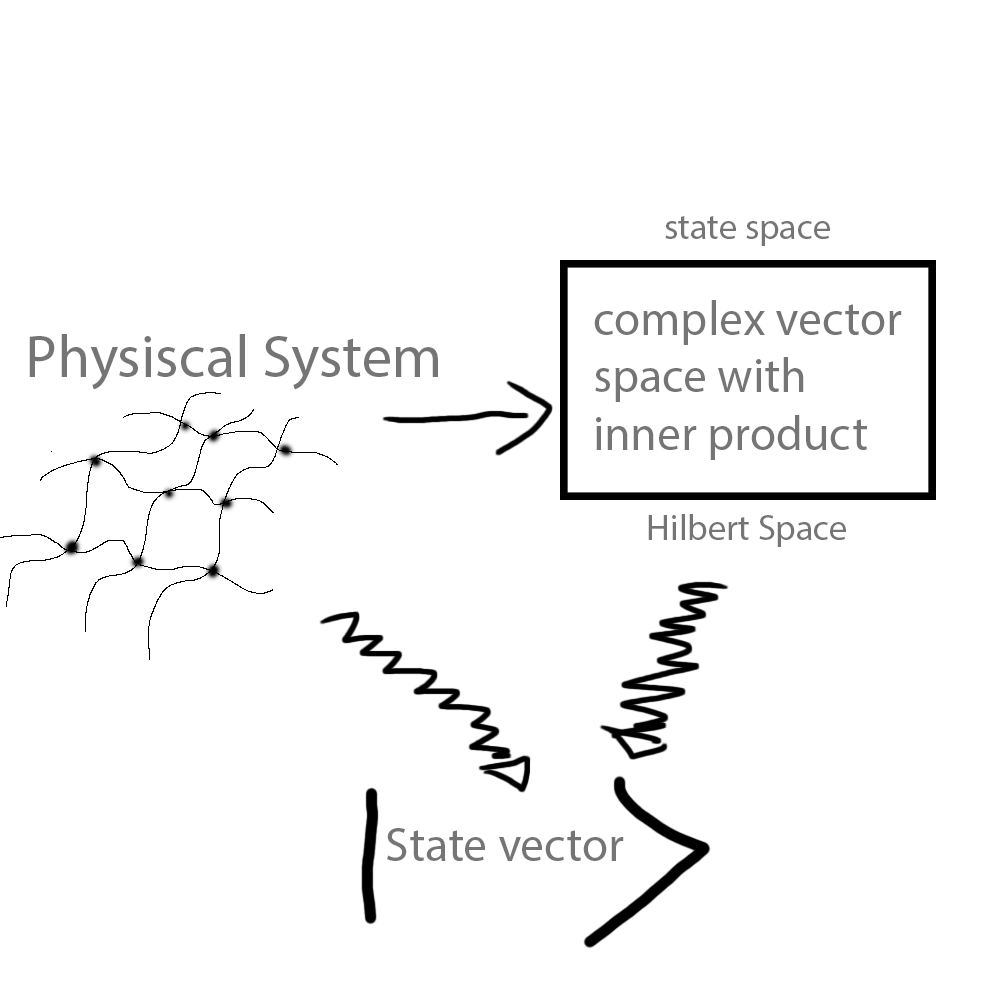
\includegraphics[scale=0.2]{images/sketch1.png} 
		\caption{how a physical state is represented}
	\end{figure}
	

	
		\subsection{Quantum Entanglement}
		%\lipsum[4]
		\begin{figure}
		\centering
		%% Little schematics showing the origin of entanglement
%% from the linear theory of QM and tensor product

\begin{tikzpicture}[scale=0.6]
  \node[colorbox=red]                      (lin)  {Linearity};
  \node[colorbox=magenta, below=.5cm of lin] (tp)  {Tensor product};
  \node[colorbox=blue, below=.5cm of tp]   (en)  {Entanglement};
  \draw[conn=2pt, densely dotted] (tp) to (lin);
  \draw[conn=2pt, densely dotted] (en) to (tp);
\end{tikzpicture}
		\caption{origin of entanglement via linearity}
		\end{figure}
		
	\section{Basics of Information Theory}
	%\lipsum[3]
		\subsection{Classical Key Agreement}
		%\lipsum[3]